\documentclass{article}

% Document extensibility %
%
% Disables native paragraph indentation
\usepackage{parskip} 
%
% Provides further bullet options for lists
\usepackage{enumitem}

% Mathematical symbol and statement packages %
%
% Necessary
\usepackage{amsmath}
\usepackage{amssymb}
%
% Extensive fraction notation
\usepackage{xfrac}
%
% Generic mathematical commands
% Notable: \degree, \celcius
\usepackage{gensymb}
%
% Variable vector notation (arrow above variable)
\usepackage{esvect}
%
% Multiline boxed equations
\usepackage{empheq}
%
% SI Unit
\usepackage{siunitx}
\usepackage{physunits}
%
% More intuitive arrays/matrices
\usepackage{array}
%
% Linear Equations
\usepackage{systeme}
%
% Boxes!
\usepackage{mdframed}

% Graphic packages %
%
% Diagrams and illustrations
\usepackage{tikz}
%
% Image insertion
\usepackage{graphicx}
\graphicspath{ {./} }

% Document content %
%
% Change title of table of contents
% \renewcommand{\contentsname}{Title}

\begin{document}

% Command `\hr` to insert horizontal rules
\newcommand{\hr}{\par\noindent\rule{\textwidth}{0.4pt}}

% Command to box and center math equations
\newcommand{\bc}[1]{
	\begin{equation*}
		\begin{boxed}
			{#1}
		\end{boxed}
	\end{equation*}
}

% Command for single line equations with a condition
\newcommand{\cond}[2]{
	\ifmmode
		{#1} \quad {#2}
	\else
		$$ {#1} \quad {#2} $$
	\fi
}

\tableofcontents

\section{Energy}

\subsection{Example}

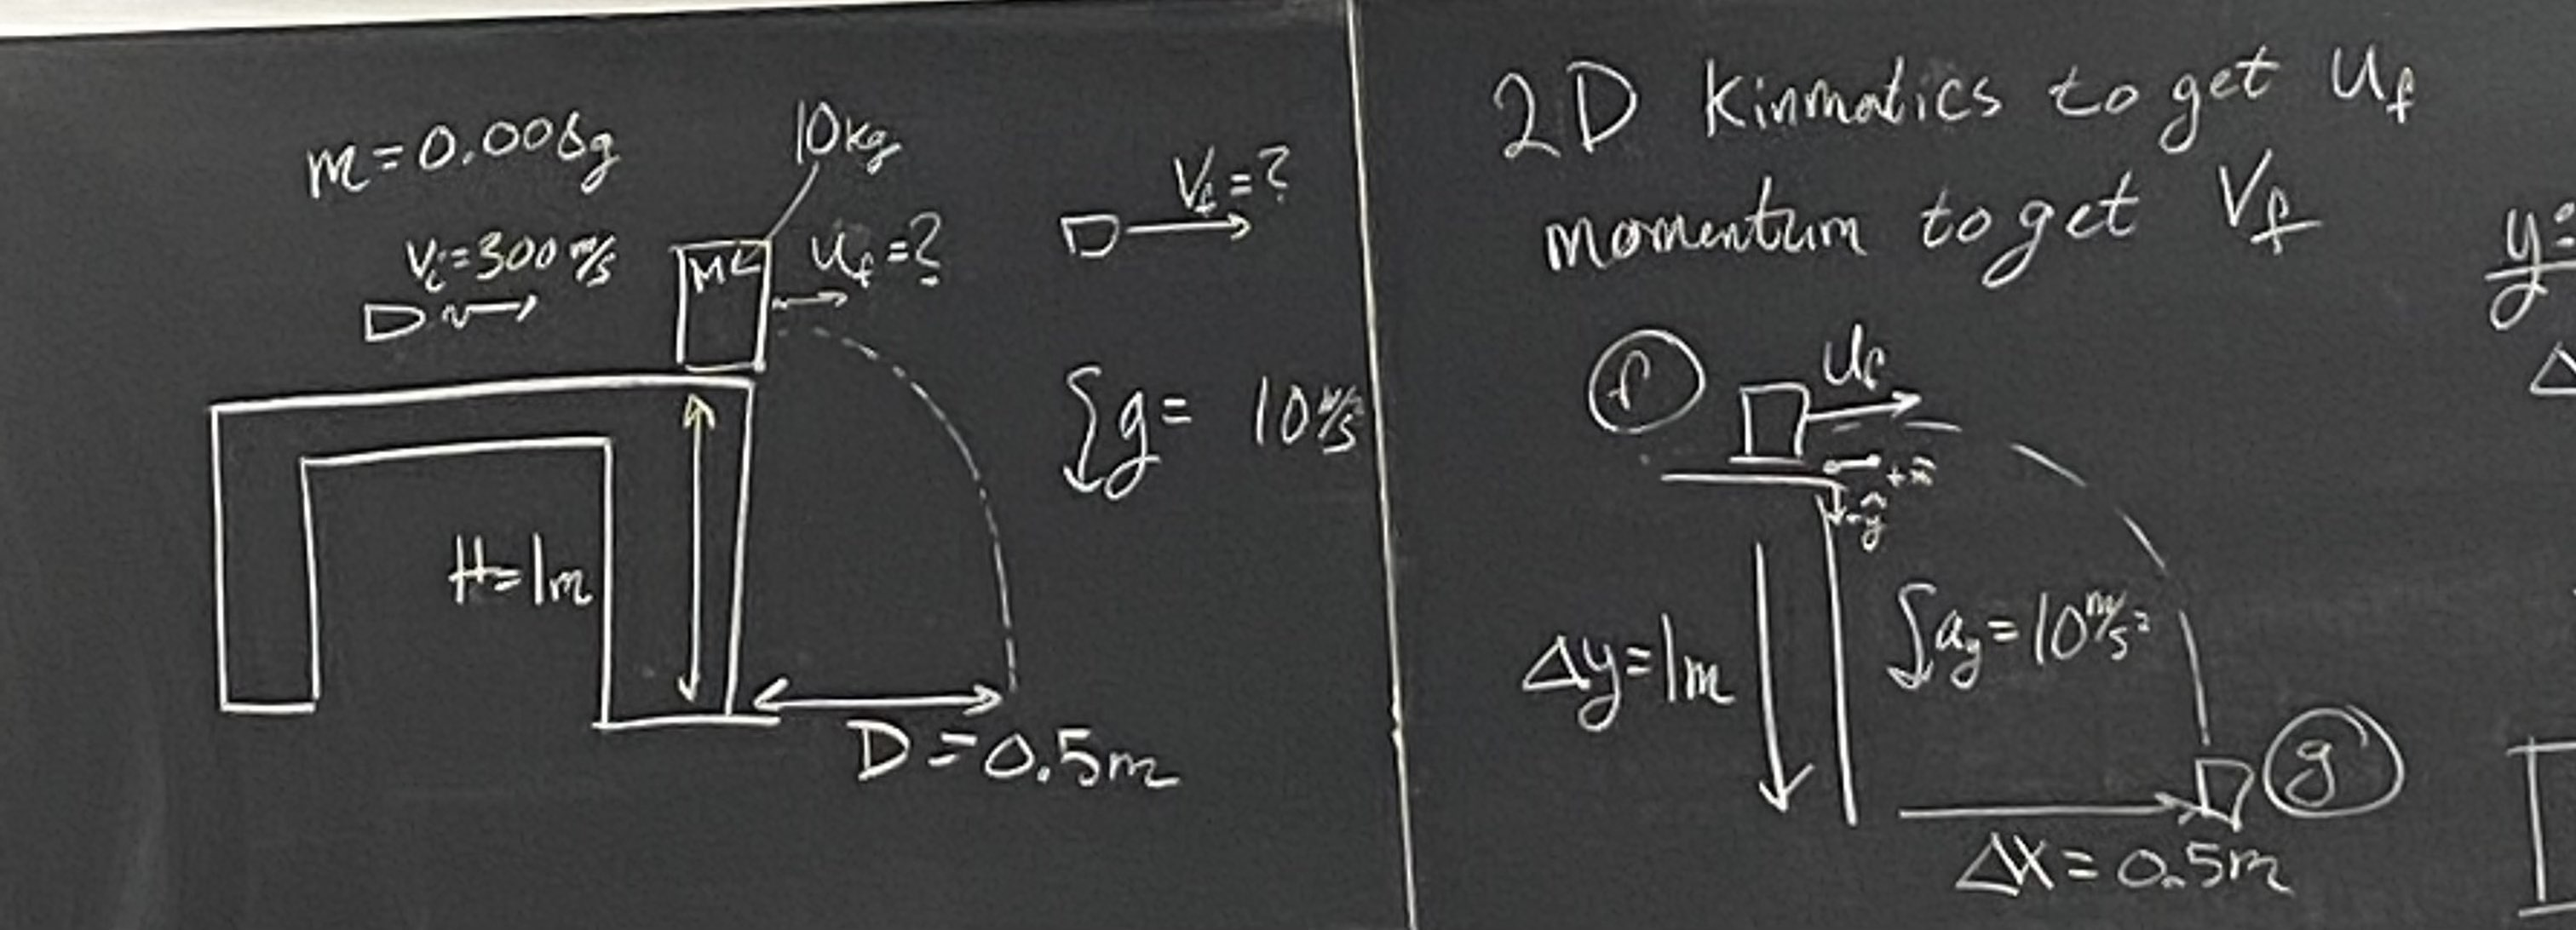
\includegraphics[width = \linewidth]{example_1.jpg}
$ \hat{y} $ Direction
\begin{align*}
	\Delta y & = v_{f_y}t + \frac{1}{2}a_yt^2 \\
	t & = \sqrt{ \frac{2\Delta y}{a_y} } \\
	t & = \sqrt{ \frac{2(\SI{1}{\meter})}{\SI{10}{\meter \per \second \squared}} } \\
	t & = \SI{0.45}{\second}
\end{align*}
$ \hat{x} $ Direction
\begin{align*}
	\Delta x & = u_{f_x}t \\
	u_{f_x} & = \frac{\Delta x}{t} \\
	u_{f_x} & = \frac{\SI{0.5}{\meter}}{\SI{0.45}{\second}} \\
	u_f & = \SI{1.11}{\meter \per \second}
\end{align*}
\begin{align*}
	\sum p_i & = \sum p_f \\
	mv_i & = Mu_f + Mv_f \\
	v_f & = \frac{mv_i - Mu_f}{m} \\
	v_f & = \frac{(\SI{8e-6}{\kilogram})(\SI{3e2}{\kilogram}) - (\SI{10}{\kilogram})(\SI{1.1}{\meter \per \second})}{\SI{8e-6}{\kilogram}} \\
	v_f & = -\SI{1e6}{\meter \per \second}
\end{align*}

\subsection{Example}

\begin{align*}
	m & = \SI{3}{\kilogram} \\
	v_i & = \SI{12}{\meter \per \second} \\
	M & = \SI{5}{\kilogram} \\
	u_i & = \SI{4}{\meter \per \second}
\end{align*}
\begin{enumerate}[label = \textbf{\arabic*)}]
	\item What is the total momentum of the system?
		\begin{align*}
			\vec{P}_i & = mv_i \hat{x} - Mu_i \hat{x} \\
			\vec{P}_i & = (\SI{36}{\kilogram \meter \per \second}) \hat{x} - (\SI{20}{\kilogram \meter \per \second}) \hat{x} \\
			\vec{P}_i & = \SI{16}{\kilogram \meter \per \second}
		\end{align*}
	\item Inelastic:
		\begin{align*}
			v_f & = ? \\
			u_f & = ?
		\end{align*}
		\begin{align*}
			P_i & = P_f \\
			mv_i - Mu_i & = (m + M)v_f \\
			v_f & = \frac{mv_i - Mu_i}{m + M} = v_{CM} \\
			v_f & = \frac{\SI{16}{\kilogram \meter \per \second}}{\SI{8}{\kilogram}} \\
			v_f & = \SI{2}{\meter \per \second} = u_f
		\end{align*}
	\item Elastic:
		\begin{align*}
			v_f & = ? \\
			u_f & = ?
		\end{align*}
		\begin{align*}
			\sum P_i & = \sum P_f \\
			mv_i - Mu_i & = -mv_f + Mu_f
		\end{align*}
		Find two unknowns ($ v_f, u_f $):
		\begin{align*}
			(\SI{3}{\kilogram})(\SI{12}{\meter \per \second}) - (\SI{5}{\kilogram})(\SI{4}{\meter \per \second}) & = -(\SI{3}{\kilogram})v_f + (\SI{5}{\kilogram})u_f \\
			-(\SI{3}{\kilogram})v_f + (\SI{5}{\kilogram})u_f & = \SI{16}{\kilogram \meter \per \second}
		\end{align*}
		\begin{align*}
			E_i & = E_f \\
			\frac{1}{2}mv_i^2 + \frac{1}{2}Mu_i^2 & = \frac{1}{2}mv_f^2 + \frac{1}{2}Mu_f^2 \\
			mv_i^2 + Mu_i^2 & = mv_f^2 + Mu_f^2 \\
			(\SI{3}{\kilogram})v_f^2 + (\SI{5}{\kilogram})u_f^2 & = (\SI{3}{\kilogram})(\SI{12}{\meter \per \second})^2 + (\SI{5}{\kilogram})(\SI{4}{\meter \per \second})^2 \\
			(\SI{3}{\kilogram})v_f^2 + (\SI{5}{\kilogram})u_f^2 & = \SI{512}{\joule}
		\end{align*}
		\begin{align*}
			-(\SI{3}{\kilogram})v_f + (\SI{5}{\kilogram})u_f & = \SI{16}{\kilogram \meter \per \second} \\
			u_f & = \SI{3.2}{\meter \per \second} + (0.6)v_f \\
			(\SI{3}{\kilogram})v_f^2 + (\SI{5}{\kilogram})(\SI{3.2}{\meter \per \second} + (0.6)v_f)^2 & = \SI{512}{\joule} \\
			(4.8)v_f^2 + 19.2v_f + 51.2 & = \SI{512}{\joule} \\
			v_f & = \SI{8}{\meter \per \second}
		\end{align*}
	\item Finding $ v_{CM} $
		\begin{align*}
			v_{CM} & = \frac{mv_i - Mu_i}{m + M} \hat{x} \\
			v_{CM} & = \frac{\SI{36}{\kilogram \meter \per \second} - \SI{20}{\kilogram \meter \per \second}}{\SI{8}{\kilogram}} \hat{x} \\
			v_{CM} & = \SI{2}{\meter \per \second} \hat{x}
		\end{align*}
		To boost into the ZMF, \underline{subtract} the vector $ v_{CM} $ from all velocities.
		\begin{tabular}{| c | c | c | c |}
			\hline
			initial & LAB & $ -v_{CM} $ & ZMF \\
			\hline
			$ \vec{v} $ & \SI{12}{\meter \per \second} & -(\SI{2}{\meter \per \second}) & \SI{10}{\meter \per \second} \\
			\hline
			$ \vec{u} $ & -\SI{4}{\meter \per \second} & -(\SI{2}{\meter \per \second}) & -(\SI{6}{\meter \per \second}) \\
			\hline
		\end{tabular}
	\item Restitution
		\begin{align*}
			m\vec{v}_f^{ZMF} & = -\epsilon m\vec{v}_i^{ZMF} \\
			\vec{v}_f^{ZMF} & = -\epsilon \vec{v}_i^{ZMF} \\
			\epsilon & = 1 \therefore \\
			\vec{v}_f^{ZMF} & = -\vec{v}_i^{ZMF} = -\SI{10}{\meter \per \second} \hat{x} \\
			\vec{u}_f^{ZMF} & = -\vec{u}_i^{ZMF} = \SI{6}{\meter \per \second} \hat{x}
		\end{align*}
		\begin{tabular}{| c | c | c | c |}
			\hline
			find & ZMF & $ v_{CM} $ & LAB \\
			\hline
			$ \vec{v} $ & -\SI{10}{\meter \per \second} & \SI{2}{\meter \per \second} & -\SI{8}{\meter \per \second} \\
			\hline
			$ \vec{u} $ & \SI{6}{\meter \per \second} & \SI{2}{\meter \per \second} & \SI{8}{\meter \per \second} \\
			\hline
		\end{tabular}
\end{enumerate}

\section{Collision}

In a free space collision which conserves momentum:
\begin{align*}
	\sum F = \frac{dp}{dt} = 0
	ma_{CM} & = 0 \rightarrow a_{CM} = 0 \\
	\frac{dv_{CM}}{dt} & = 0 \rightarrow v_{CM} = \text{constant}
\end{align*}

The problems for momentum are usually given in the LAB frame (lit. in the laboratory), however if we co-more with the center of mass momentum problems become trivial. This frame is the \underline{Zero Momentum Frame} or \underline{ZMF}.

To find the ZMF,
\begin{equation} v_{CM} = \frac{\sum \vec{P}}{\sum m} \end{equation}

\hr

\begin{equation}
	\vec{P}_f^{ZMF} = -\epsilon \vec{P}_i^{ZMF}
\end{equation}
\underline{Coefficient of Restitution} - a description of how much the relative speed changes in a collision.
\begin{itemize}
	\item Means relative speed is fully conserved.
		$$ \epsilon = 1 $$
	\item Means $ v_{ref_f} = 0 $
		$$ \epsilon = 0 $$
	\item Reflects some speed loss.
		$$ 0 < \epsilon < 1 $$
\end{itemize}

\subsection{Example}

Two masses collide head-on
\begin{align*}
	m & = \SI{3}{\kilogram} \\
	v_i & = \SI{5}{\meter \per \second} \\
	M & = \SI{5}{\kilogram} \\
	u_i & = \SI{8}{\meter \per \second}
\end{align*}
Find final speeds, elastic, inelastic, $ \epsilon = 0.4 $.
\begin{enumerate}[label = \textbf{\arabic*)}]
	\item Final Speeds
		\begin{align*}
			\sum P_i & = \sum P_f \\
			mv_i - Mu_i & = -mv_f + Mu_f \\
			(\SI{3}{\kilogram})(\SI{5}{\meter \per \second}) - (\SI{5}{\kilogram})(\SI{8}{\meter \per \second}) & = -(\SI{3}{\kilogram})v_f + (\SI{5}{\kilogram})u_f \\
			-(\SI{3}{\kilogram})v_f + (\SI{5}{\kilogram})u_f & = -\SI{25}{\kilogram \meter \per \second} \\
			u_f & = -\SI{5}{\meter \per \second} + (0.6)v_f
		\end{align*}
		\begin{align*}
			E_i & = E_f \\
			mv_i^2 + Mu_i^2 & = mv_f^2 + Mu_f^2 \\
			(\SI{3}{\kilogram})(\SI{5}{\meter \per \second})^2 + (\SI{5}{\kilogram})(\SI{8}{\meter \per \second})^2 & = (\SI{3}{\kilogram})v_f^2 + (\SI{5}{\kilogram})u_f^2 \\
			(\SI{3}{\kilogram})v_f^2 + (\SI{5}{\kilogram})u_f^2 & = \SI{395}{\joule}
		\end{align*}
		\begin{align*}
			(\SI{3}{\kilogram})v_f^2 + (\SI{5}{\kilogram})(-\SI{5}{\meter \per \second} + (0.6)v_f)^2 & = \SI{395}{\joule} \\
			(4.8)v_f^2 - (30)v_f + 125 & = \SI{395}{\joule} \\
			v_f & = \SI{11.25}{\meter \per \second}, -\SI{5.0}{\meter \per \second}
		\end{align*}
		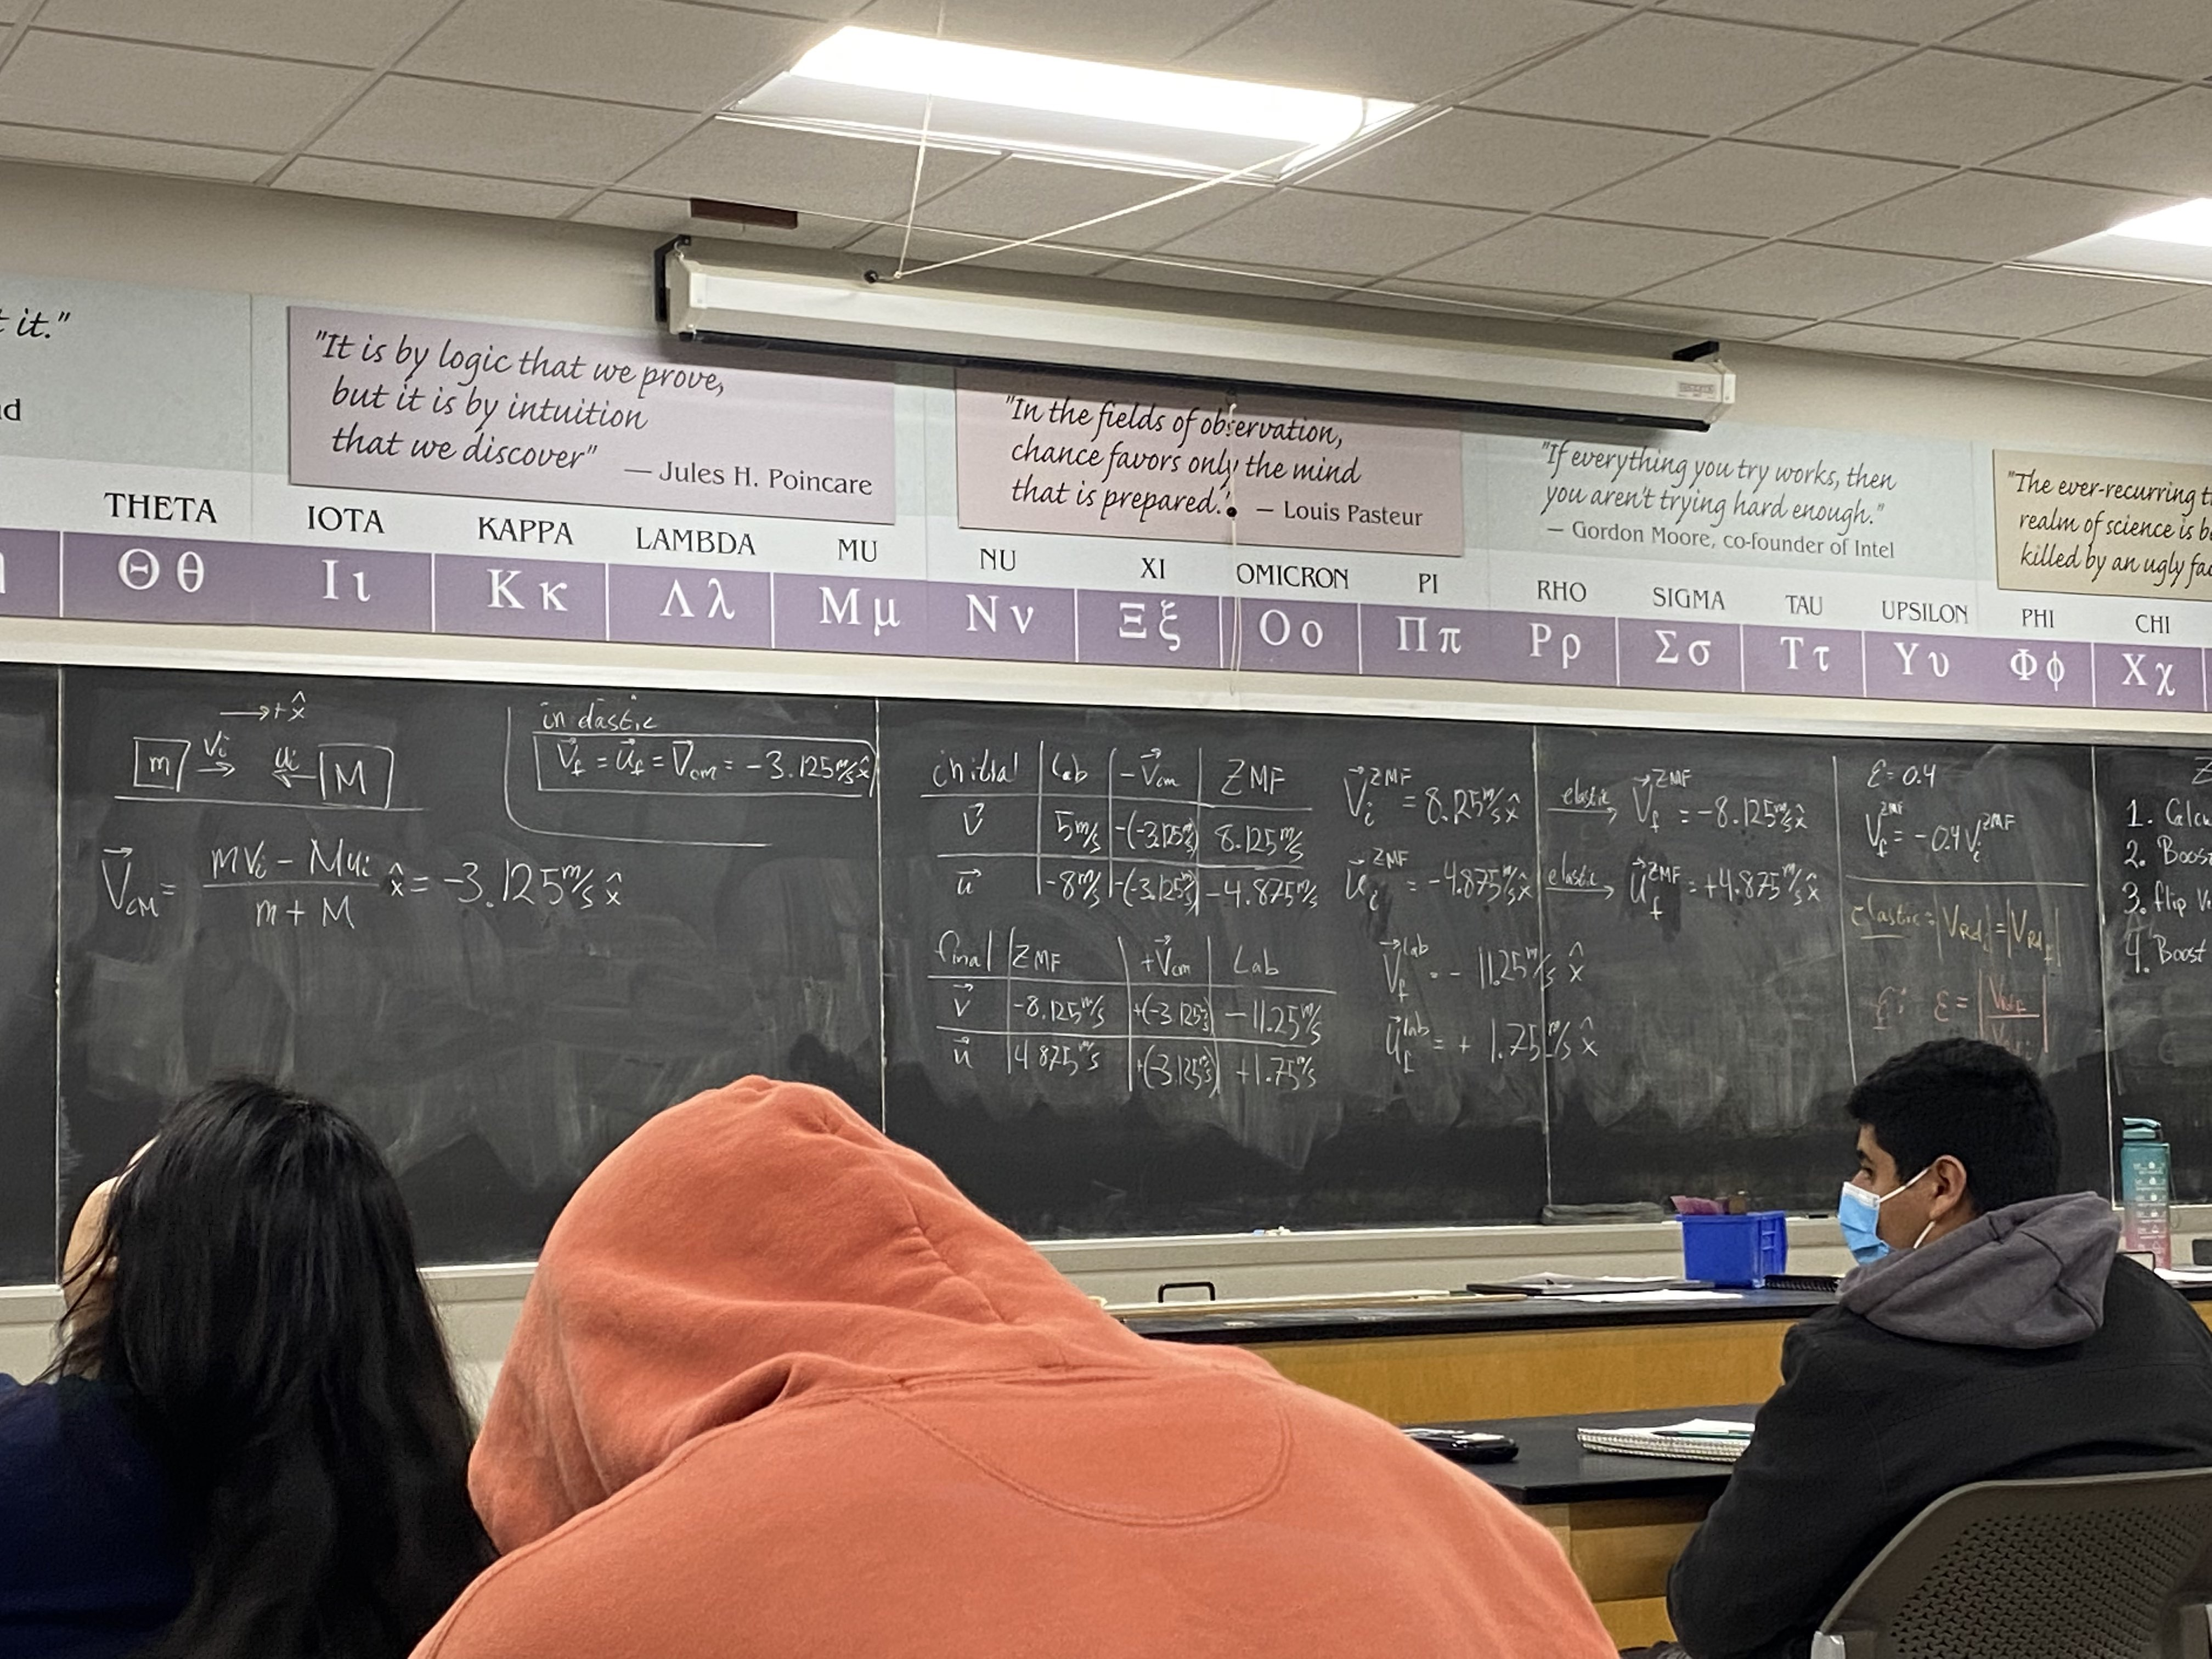
\includegraphics[width = \linewidth]{example_2.jpg}
\end{enumerate}

\end{document}
